Deviations of the population distribution from normality depend on the
distribution of coalescent times and the genetic parameters. One natural way to
quantify a distribution's deviation from normality is through its kurtosis. The
kurtosis, defined as $M_4/M_2^2$, measures the tendency of a
distribution to produce outliers \citep{Westfall2014}. However, since the
kurtosis is a ratio of two random variables, its expectation is challenging to
calculate. Rather than attempt this calculation, we compare the expected fourth
central moment itself to that expected under normality. This approach
qualitatively identifies the factors influencing deviations from normality.

Using the low mutation rate approximation, the ratio of the expected fourth
moment to that under normality simplifies to
\begin{equation}
  \label{eq:popmom4coal}
  \frac{\E[M_4]}{3\left(L \T \E[\mathbbm{T}_{2,2}] m_2\right)^2} \approx 1 +
  \underbrace{\frac{m_4}{m_2^2}}_{\text{mutation}} \underbrace{(6 L \T \E[\mathbbm{T}_{2,2}])^{-1}}_{\text{sparsity}}
      \underbrace{\left( \frac{2\E[\mathbbm{T}_{4,4}] +
      \frac{2}{3}\E[\mathbbm{T}_{3,4}] +
      \frac{4}{9}\E[\mathbbm{T}_{2,4}]}{\E[\mathbbm{T}_{2,2}]}\right)}_{\text{demography}}
  %\frac{m_2/m_4}{6 L \T \E[\mathbbm{T}_{2,2}]}\left( \frac{2\E[\mathbbm{T}_{4,4}] +
  %    \frac{2}{3}\E[\mathbbm{T}_{3,4}] +
  %    \frac{4}{9}\E[\mathbbm{T}_{2,4}]}{\E[\mathbbm{T}_{2,2}]}\right),
\end{equation}
The expected excess in $M_4$, relative to normality, increases with sparsity and
with $m_4/m_2^2$. $m_4/m_2^2$ is equal to the kurtosis of the mutational effect
distribution when mutations are unbiased and reflects its propensity to produce
large effect mutations. The excess depends on demography through the factor $Q
= \frac{2\E[\mathbbm{T}_{4,4}] + \frac{2}{3}\E[\mathbbm{T}_{3,4}]
+ \frac{4}{9}\E[\mathbbm{T}_{2,4}]}{\E[\mathbbm{T}_{2,2}]}$. The extent to which
demography increases or decreases deviations from normality can be investigated
by calculating $Q$ in different models. In a constant-size and panmictic
population $Q$ is equal to one. In a population where lineages are exchangeable,
$\E[\mathbbm{T}_{k,n}]$ can be calculated numerically using expressions from
\citet{Griffiths1998} or \citet{Polanski2003a}. Values of $Q$ in an exponentially growing population are
shown in Figure \ref{fig:Qexp}A. Holding sparsity and the mutational
distribution constant, a population which underwent exponential growth will have
a greater expected deviation from normality in its trait distribution. Another
example demography is a population that goes through a step change at some point
in the past. Figure \ref{fig:Qexp}B shows that when the population size
increased at some point in the past, $Q$ is increased similarly to the
exponential growth scenario. When the population experiences a bottleneck $Q$ is
decreased below one. Additionally, $Q$ appears more sensitive to population
growth than to bottlenecks.

\begin{figure}
\centering
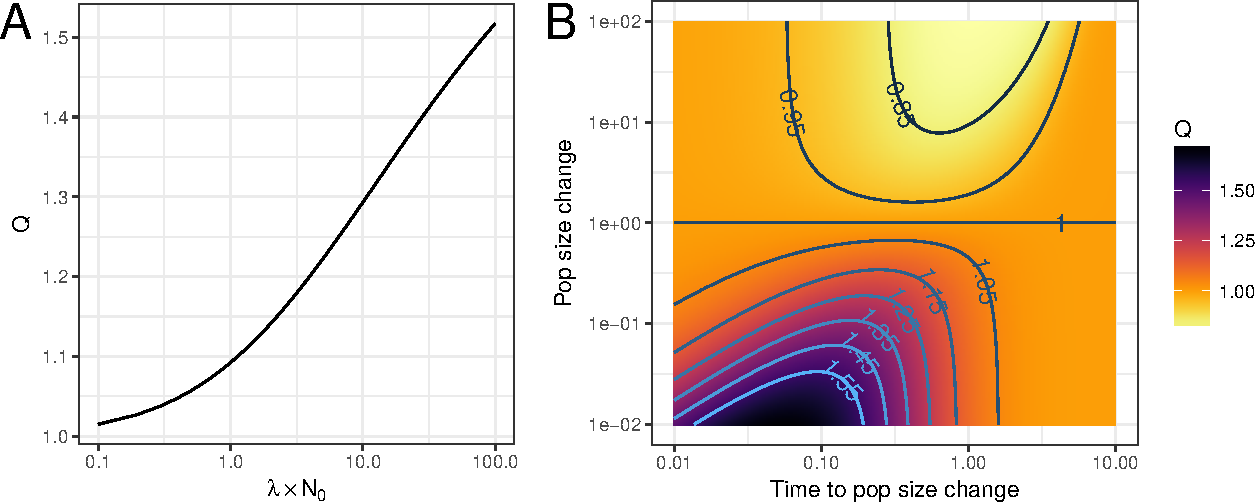
\includegraphics[width=\textwidth]{./figures/combo_q.pdf}

\caption{
\textbf{The effects of demography on deviations of the expected
fourth central moment of the population trait distribution from normality.} $Q$
measures the effect due to demography on the expected fourth central moment
(equation \eqref{eq:popmom4coal}). (\textbf{A}): $Q$ increases as the
exponential growth rate increases relative to the current population
size.~$\lambda$ is the growth rate and $N_0$ is the initial effective population
size.~(\textbf{B}): $Q$ values when the population undergoes an instantaneous
step change at some point in the past. The time and magnitude of this change are
given in units of the current effective population size. $Q$ increases when the
population grows and decreases when it declines.}

\label{fig:Qexp}
\end{figure}

\begin{figure}
\centering
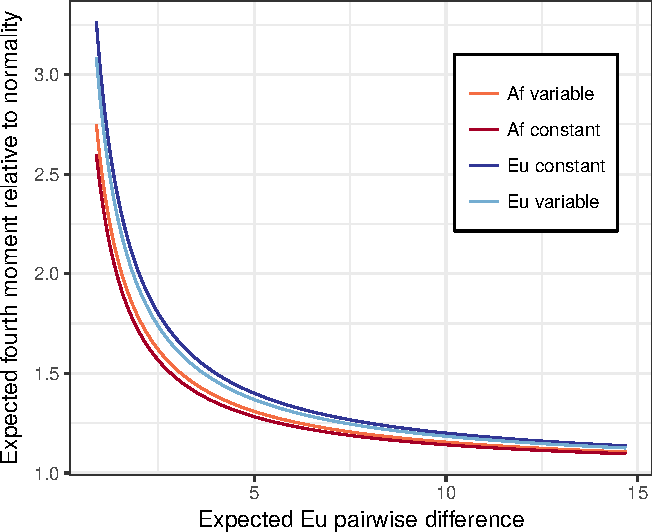
\includegraphics[width=0.55\textwidth]{./figures/af_eu_mom4_r.pdf}
\caption{ \textbf{A comparison between the expected fourth moment at different levels of
sparsity in the African and European demographic models fit
by \citet{Tennessen2012}.} Trait sparsity is varied by changing the expected
number pairwise differences at sites affecting the trait in the European model.
The mutational kurtosis is set to six. The darker lines show the predicted
relationship for populations with the same heterozygosity as the European and
African models but with constant size.}
\label{fig:afeucomp}
\end{figure}

As a concrete example, we can consider the differences in the expected fourth
moment produced by different demographic histories in different human
populations. In the demographic model fit by \citet{Tennessen2012}, the generic
European population experiences a bottleneck associated with out-of-Africa and
recent growth while the generic African population experiences a more stable
history also with recent growth. Differences in demographic history between the
two populations has resulted in a lower heterozygosity in European populations
due to the out-of-Africa bottleneck \citep{Yu2002}.

For a given sparsity, the African population model predicts a smaller deviation
from normality than the European model (Figure \ref{fig:afeucomp}). The expected
fourth moment in constant-size populations with the same heterozygosity as the
African and European models is lower for the African model and higher for the
European model. This is because the African model is dominated by population
growth that leads to a $Q$ greater than one, while the European model is
dominated by a bottleneck event that leads to a $Q$ less than one
(Figure \ref{fig:Qexp}). However, differences due to demography are small and
deviations from normality are mostly driven by differences in heterozygosity at
causal loci.

Even though recombination is not included in the model, we can form an idea
about how linkage might impact deviations from normality. Line two of
equation \eqref{eq:emoms4} corresponds to the contribution from two mutations
occurring at a single locus. The first quantity indicates that the expectation
of the fourth moment increases with the variance of the pairwise coalescence
time. The second part does not have a clear interpretation. If the sum of these
two terms is positive this agrees with the intuition that linkage disequilibrium
increases deviations from normality by reducing the effective number of
independent loci.

Simulations of the kurtosis itself show substantial variance, with about a
quarter of simulated populations having a value less than three (that of a
normal distribution) even as the mean kurtosis increases to almost nine
(Appendix \ref{kurtsim}). This high variance in the kurtosis is likely due to a
high variance in both the trait variance and fourth moment. This, along with the
fact that deviations from the infinitesimal model inflate the fourth moment
(equation \eqref{eq:popmom4coal}), leads to a situation where the kurtosis
increases with trait sparsity but the variance is high across evolutionary
realizations.
%%% Local Variables:
%%% TeX-master: "quant_gen_manu.tex"
%%% End:
